\section{Introduction}

The OpenMPI library implements several algorithms to perform collective blocking operations according to many different parameters.
OSU Micro-Benchmark is a tool that allows us to evaluate the performance of these operations.

\subsection{Computational architecture}

In order to test the performance of the broadcast and reduce operations, we will use a high-performance computing cluster. The computational resources used to complete the assignment are the ones provided by the ORFEO cluster.

The ORFEO system architecture consists of different machines architecture, in this project the THIN partition is used. The THIN partition consist of 12 Intel nodes: two equipped with Xeon Gold 6154 and 10 equipped with Xeon Gold 6126 cpus.

\subsection{OSU Micro-Benchmark}

OMB includes benchmarks for various MPI blocking
collective operations (Allgather, Alltoall,Allreduce, Barrier, Bcast, Gather, Reduce, Reduce-Scatter, Scatter and vector collectives). These benchmarks work in the following manner. Suppose users run the osu Bcast benchmark with N processes, the benchmark measures the min, max and the average latency of the MPI\_Bcast collective operation across N processes, for various message lengths, over a large number of iterations. In our experiments, we will consider the average latency for each message length.

In this report, two operations are take into consideration: broadcast and reduce.


\subsection{Broadcast}

The broadcast operation \texttt{MPI\_Bcast} is a one-to-all communication operation which allows a process (typically the root process) to distribute information across many processes. This operation is implemented in OpenMP using different algorithms. The algorithms that are considered in this analysis are:
\begin{itemize}
    \item \textbf{basic linear}, the root process sends to all the other process the message without segmentation;
    \begin{center}
    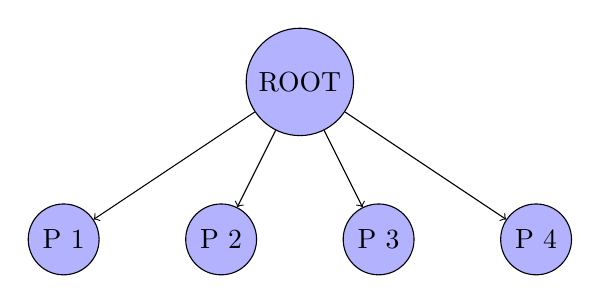
\begin{tikzpicture}
        [
        level distance=2cm,
        sibling distance=2cm,
        every node/.style={circle, draw, fill=blue!30},
        edge from parent/.style={->,draw}
        ]
        % Root node
        \node {ROOT}
        % Level 1: Children nodes
        child { node {P 1} }
        child { node {P 2} }
        child { node {P 3} }
        child { node {P 4} };
    \end{tikzpicture}
    \end{center}

    \item \textbf{chain}, the message is split into segments and transmission of segments continues in a pipeline until the last node gets the broadcast message. ith process receives the message from the $(i-1)$-th process, and sends it to $(i+1)$-th process;
    
    \begin{center}
    \begin{tikzpicture}[
        every node/.style={circle, draw, fill=blue!30},
        <-, >=stealth
        ]
        % Define the nodes
        \node (n1) {P 3};
        \node (n2) [right=of n1] {P 2};
        \node (n3) [right=of n2] {P 1};
        \node (n4) [right=of n3] {ROOT};
      
        % Draw the arrows
        \draw (n1) -- (n2);
        \draw (n2) -- (n3);
        \draw (n3) -- (n4);
    \end{tikzpicture}
    \end{center}

    \item \textbf{split binary tree}, suppose that each process is a node of a binary tree and the root node is the root process, each parent node sends the message to its children. As the name of the algorithm suggests, the message is split in two halves before transmission and when each half of the message reaches its destination, it is necessary to merge the two halves.
    \begin{center}
        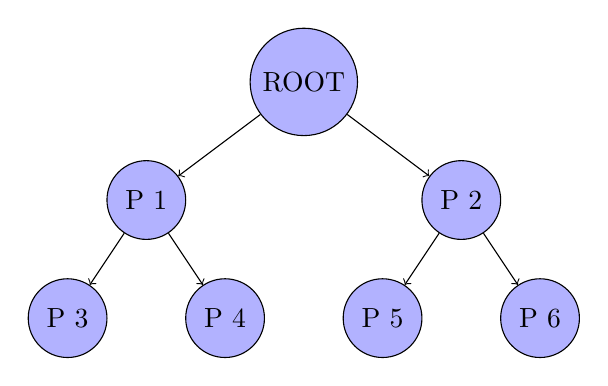
\begin{tikzpicture}[
            level 1/.style={sibling distance=4cm},
            level 2/.style={sibling distance=2cm},
            every node/.style={circle, draw, fill=blue!30, minimum size=1cm},
            edge from parent/.style={->, draw}
            ]
            % Root node
            \node {ROOT}
              % Level 1
              child { node {P 1}
                % Level 2
                child { node {P 3} }
                child { node {P 4} }
              }
              child { node {P 2}
                % Level 2
                child { node {P 5} }
                child { node {P 6} }
              };
          \end{tikzpicture}
    \end{center}

\end{itemize}


\subsection{Reduce}

The reduce operation \texttt{MPI\_Reduce} combines the elements provided in the input buffer of each process in the grouping the specified operation, and returns the combined value in the output buffer of the root process. The specific operation used to reduce the input in the OSU benchmark are sum, maximum, and minimum.

The algorithms that are considered in this analysis are:
\begin{itemize}
    \item \textbf{basic linear }, the root process receives the message from all the other process and reduces the messages;
    \item \textbf{chain}, if we order the processes with respect to their rank, each process sends the message to the next process, each process receives the message from the previous process and reduces the messages;
    \item \textbf{binary tree }, suppose that each process is a node of a binary tree and the root node is the root process. Each parent node receives the message from its children and reduces the received messages passing the result to its parent node.
\end{itemize}